\chapter{Additional Plots}
\label{appndx:plots}
\section*{Parameter Analysis}
\begin{figure}[htbp] 
    \begin{center}
        \begin{tabular}{cc}
            
            \hspace{-5mm} \resizebox{80mm}{!}{\includegraphics{res/{1-rnd-speed-kappa}.pdf}} &
            \hspace{-10mm} \resizebox{80mm}{!}{\includegraphics{res/{1-vs-speed-kappa}.pdf}} \\
            \scriptsize{(c)} & \scriptsize{(f)} \\
            
        \end{tabular}
        \caption{Effect of drift coefficient on performance (a-c) random RBF (d-f) VS RBF}
        \label{fig:apndeffect:speed1}
    \end{center}
\end{figure}

\begin{figure}[htbp] 
    \begin{center}
        \begin{tabular}{cc}
            \hspace{-5mm} \resizebox{80mm}{!}{\includegraphics{res/{1-rnd-speed-depth}.pdf}} &
            \hspace{-10mm} \resizebox{80mm}{!}{\includegraphics{res/{1-vs-speed-depth}.pdf}} \\
            \scriptsize{(a)} & \scriptsize{(d)} \\
            
        \end{tabular}
        \caption{Effect of drift coefficient on structure (a-c) random RBF (d-f) VS RBF}
        \label{fig:apndeffect:speed2}
    \end{center}
\end{figure}
\begin{figure}[htbp] 
    \begin{center}
        \begin{tabular}{cc}
            
            \hspace{-5mm} \resizebox{80mm}{!}{\includegraphics{res/{1-rnd-speed-tsize}.pdf}} &
            \hspace{-10mm} \resizebox{80mm}{!}{\includegraphics{res/{1-vs-speed-tsize}.pdf}} \\
            \scriptsize{(b)} & \scriptsize{(e)} \\
            
        \end{tabular}
        \caption{Effect of drift coefficient on structure (a-c) random RBF (d-f) VS RBF}
        \label{fig:apndeffect:speed2}
    \end{center}
\end{figure}
\begin{figure}[htbp] 
    \begin{center}
        \begin{tabular}{ccc}
            \hspace{-5mm} \resizebox{80mm}{!}{\includegraphics{res/{1-rnd-speed-memory}.pdf}} &
            \hspace{-10mm} \resizebox{80mm}{!}{\includegraphics{res/{1-vs-speed-memory}.pdf}} \\
            \scriptsize{(c)} & \scriptsize{(f)} \\
            
        \end{tabular}
        \caption{Effect of drift coefficient on structure (a-c) random RBF (d-f) VS RBF}
        \label{fig:apndeffect:speed2}
    \end{center}
\end{figure}




\begin{figure}[htbp] 
    \begin{center}
        \begin{tabular}{cc}
            \hspace{-5mm} \resizebox{80mm}{!}{\includegraphics{res/{2-rnd-grace-depth}.pdf}} &
            \hspace{-10mm} \resizebox{80mm}{!}{\includegraphics{res/{2-vs-grace-depth}.pdf}} \\
            \scriptsize{(a)} & \scriptsize{(d)} \\
            
            
        \end{tabular}
        \caption{Effect of grace period on structure (a-c) random RBF (d-f) VS RBF}
        \label{fig:apndeffect:grace2}
    \end{center}
\end{figure}

\begin{figure}[htbp] 
    \begin{center}
        \begin{tabular}{cc}
            
            \hspace{-5mm} \resizebox{80mm}{!}{\includegraphics{res/{2-rnd-grace-memory}.pdf}} &
            \hspace{-10mm} \resizebox{80mm}{!}{\includegraphics{res/{2-vs-grace-memory}.pdf}} \\
            \scriptsize{(c)} & \scriptsize{(f)} \\
            
        \end{tabular}
        \caption{Effect of grace period on structure (a-c) random RBF (d-f) VS RBF}
        \label{fig:apndeffect:grace2}
    \end{center}
\end{figure}



\begin{figure}[htbp] 
    \begin{center}
        \begin{tabular}{cc}
            
            \hspace{-5mm} \resizebox{80mm}{!}{\includegraphics{res/{3-rnd-centroid-memory}.pdf}} &
            \hspace{-10mm} \resizebox{80mm}{!}{\includegraphics{res/{3-vs-centroid-memory}.pdf}} \\
            \scriptsize{(c)} & \scriptsize{(f)} \\
            
        \end{tabular}
        \caption{Effect of number of centroids on structure (a-c) random RBF (d-f) VS RBF}
        \label{fig:apndeffect:centroid2}
    \end{center}
\end{figure}



\begin{figure}[htbp] 
    \begin{center}
        \begin{tabular}{cc}
            
            \hspace{-5mm} \resizebox{80mm}{!}{\includegraphics{res/{4-rnd-driftcentroid-time}.pdf}} &
            \hspace{-10mm} \resizebox{80mm}{!}{\includegraphics{res/{4-vs-driftcentroid-time}.pdf}} \\
            \scriptsize{(b)} & \scriptsize{(e)} \\
            
        \end{tabular}
        \caption{Effect of percentage of drift centroids on performance (a-c) random RBF (d-f) VS RBF}
        \label{fig:apndeffect:driftcentroid1}
    \end{center}
\end{figure}
\begin{figure}[htbp] 
    \begin{center}
        \begin{tabular}{cc}
            \hspace{-5mm} \resizebox{80mm}{!}{\includegraphics{res/{4-rnd-driftcentroid-tsize}.pdf}} &
            \hspace{-10mm} \resizebox{80mm}{!}{\includegraphics{res/{4-vs-driftcentroid-tsize}.pdf}} \\
            \scriptsize{(b)} & \scriptsize{(e)} \\
            
            
        \end{tabular}
        \caption{Effect of percentage of drift centroids on structure (a-c) random RBF (d-f) VS RBF}
        \label{fig:apndeffect:driftcentroid2}
    \end{center}
\end{figure}
\begin{figure}[htbp] 
    \begin{center}
        \begin{tabular}{cc}
            
            \hspace{-5mm} \resizebox{80mm}{!}{\includegraphics{res/{4-rnd-driftcentroid-memory}.pdf}} &
            \hspace{-10mm} \resizebox{80mm}{!}{\includegraphics{res/{4-vs-driftcentroid-memory}.pdf}} \\
            \scriptsize{(c)} & \scriptsize{(f)} \\
            
        \end{tabular}
        \caption{Effect of percentage of drift centroids on structure (a-c) random RBF (d-f) VS RBF}
        \label{fig:apndeffect:driftcentroid2}
    \end{center}
\end{figure}



\begin{figure}[htbp] 
    \begin{center}
        \begin{tabular}{cc}
            
            \hspace{-5mm} \resizebox{80mm}{!}{\includegraphics{res/{5-rnd-tiethresh-time}.pdf}} &
            \hspace{-10mm} \resizebox{80mm}{!}{\includegraphics{res/{5-vs-tiethresh-time}.pdf}} \\
            \scriptsize{(b)} & \scriptsize{(e)} \\
            
            
        \end{tabular}
        \caption{Effect of tie threshold on performance (a-c) random RBF (d-f) VS RBF}
        \label{fig:apndeffect:tiethresh1}
    \end{center}
\end{figure}
\clearpage

\begin{figure}[htbp] 
    \begin{center}
        \begin{tabular}{cc}
            \hspace{-5mm} \resizebox{80mm}{!}{\includegraphics{res/{5-rnd-tiethresh-depth}.pdf}} &
            \hspace{-10mm} \resizebox{80mm}{!}{\includegraphics{res/{5-vs-tiethresh-depth}.pdf}} \\
            \scriptsize{(a)} & \scriptsize{(d)} \\
            
        \end{tabular}
        \caption{Effect of tie threshold on structure (a-c) random RBF (d-f) VS RBF}
        \label{fig:apndeffect:tiethresh2}
    \end{center}
\end{figure}

\begin{figure}[htbp] 
    \begin{center}
        \begin{tabular}{cc}
            \hspace{-5mm} \resizebox{80mm}{!}{\includegraphics{res/{6-rnd-binsplit-accu}.pdf}} &
            \hspace{-10mm} \resizebox{80mm}{!}{\includegraphics{res/{6-vs-binsplit-accu}.pdf}} \\
            \scriptsize{(a)} & \scriptsize{(d)} \\
            
        \end{tabular}
        \caption{Effect of binary split centroids on performance (a-c) random RBF (d-f) VS RBF}
        \label{fig:apndeffect:binsplit1}
    \end{center}
\end{figure}



\begin{figure}[H]
    \begin{center}
        \begin{tabular}{cc}
            \hspace{-5mm} \resizebox{80mm}{!}{\includegraphics{res/{6-rnd-binsplit-time}.pdf}} &
            \hspace{-10mm} \resizebox{80mm}{!}{\includegraphics{res/{6-vs-binsplit-time}.pdf}} \\
            \scriptsize{(b)} & \scriptsize{(e)} \\
            
        \end{tabular}
        \caption{Effect of binary split centroids on performance (a-c) random RBF (d-f) VS RBF}
        \label{fig:apndeffect:binsplit1}
    \end{center}
\end{figure}


\begin{figure}[htbp] 
    \begin{center}
        \begin{tabular}{cc}
            
            \hspace{-5mm} \resizebox{80mm}{!}{\includegraphics{res/{6-rnd-binsplit-memory}.pdf}} &
            \hspace{-10mm} \resizebox{80mm}{!}{\includegraphics{res/{6-vs-binsplit-memory}.pdf}} \\
            \scriptsize{(c)} & \scriptsize{(f)} \\
            
        \end{tabular}
        \caption{Effect of binary split on structure (a-c) random RBF (d-f) VS RBF}
        \label{fig:apndeffect:binsplit2}
    \end{center}
\end{figure}


\begin{figure}[htbp] 
    \begin{center}
        \begin{tabular}{cc}
            \hspace{-5mm} \resizebox{80mm}{!}{\includegraphics{res/{7-rnd-maxsize-accu}.pdf}} &
            \hspace{-10mm} \resizebox{80mm}{!}{\includegraphics{res/{7-vs-maxsize-accu}.pdf}} \\
            \scriptsize{(a)} & \scriptsize{(d)} \\
            
            
        \end{tabular}
        \caption{Effect of maximum allowed size of tree on performance (a-c) random RBF (d-f) VS RBF}
        \label{fig:apndeffect:maxsize1}
    \end{center}
\end{figure}
\begin{figure}[H] 
    \begin{center}
        \begin{tabular}{cc}
            \hspace{-5mm} \resizebox{80mm}{!}{\includegraphics{res/{8-rnd-ensize-depth}.pdf}} &
            \hspace{-10mm} \resizebox{80mm}{!}{\includegraphics{res/{8-vs-ensize-depth}.pdf}} \\
            \scriptsize{(a)} & \scriptsize{(d)} \\
            
            
        \end{tabular}
        \caption{Effect of ensemble size on structure (a-c) random RBF (d-f) VS RBF}
        \label{fig:apndeffect:ensize2}
    \end{center}
\end{figure}
\begin{figure}[htbp] 
    \begin{center}
        \begin{tabular}{cc}
            
            \hspace{-5mm} \resizebox{80mm}{!}{\includegraphics{res/{8-rnd-ensize-tsize}.pdf}} &
            \hspace{-10mm} \resizebox{80mm}{!}{\includegraphics{res/{8-vs-ensize-tsize}.pdf}} \\
            \scriptsize{(b)} & \scriptsize{(e)} \\
            
            
        \end{tabular}
        \caption{Effect of ensemble size on structure (a-c) random RBF (d-f) VS RBF}
        \label{fig:apndeffect:ensize2}
    \end{center}
\end{figure}

\begin{figure}[htbp] 
    \begin{center}
        \begin{tabular}{cc}
            \hspace{-5mm} \resizebox{80mm}{!}{\includegraphics{res/{9-rnd-ifreset-accu}.pdf}} &
            \hspace{-10mm} \resizebox{80mm}{!}{\includegraphics{res/{9-vs-ifreset-accu}.pdf}} \\
            \scriptsize{(a)} & \scriptsize{(d)} \\
            
        \end{tabular}
        \caption{Effect of tree reset (within ensemble) on performance (a-c) random RBF (d-f) VS RBF}
        \label{fig:apndeffect:ifreset1}
    \end{center}
\end{figure}


\begin{figure}[htbp] 
    \begin{center}
        \begin{tabular}{cc}
            \hspace{-5mm} \resizebox{80mm}{!}{\includegraphics{res/{10-rnd-firsttree-accu}.pdf}} &
            \hspace{-10mm} \resizebox{80mm}{!}{\includegraphics{res/{10-vs-firsttree-accu}.pdf}} \\
            \scriptsize{(a)} & \scriptsize{(d)} \\
            
            
        \end{tabular}
        \caption{Effect of first tree size centroids on performance (a-c) random RBF (d-f) VS RBF}
        \label{fig:apndeffect:firsttree1}
    \end{center}
\end{figure}

\clearpage
\section*{Comparative Analysis Over Timeline}

\begin{figure}[htbp] 
    \begin{center}
        \begin{tabular}{cc}
            \hspace{-5mm} \resizebox{80mm}{!}{\includegraphics{resw/{1-rnd-count-time}.pdf}} &
            \hspace{-10mm} \resizebox{80mm}{!}{\includegraphics{resw/{1-vs-count-time}.pdf}} \\
            \scriptsize{(a)} & \scriptsize{(d)} \\
            
            \hspace{-5mm} \resizebox{80mm}{!}{\includegraphics{resw/{1-rnd-count-tsize}.pdf}} &
            \hspace{-10mm} \resizebox{80mm}{!}{\includegraphics{resw/{1-vs-count-tsize}.pdf}} \\
            \scriptsize{(b)} & \scriptsize{(e)} \\
            
        \end{tabular}
        \caption{(a,d) time, (b,e) tree size, (c,f) kappa values over time for (a-c) random RBF, (d-f) VS RBF}
        \label{fig:apndeffect:wintime}
    \end{center}
\end{figure}

\clearpage


\chapter{Extended Related Works}
\label{appndx:erw}
In a recent approach, \cite{rutkowski13:vfdt} argued that using McDiarmid’s bound instead of Hoeffding bound in VFDT is more appropriate for ensuring the approximation bound i.e. the split decisions made after seeing certain number of instances will, with high probability, remain the same for infinite number of instances. The authors also presented McDiarmid’s bound for information gain of ID3 algorithm, and Gini index of CART algorithm. It is to be noted that Hoeffding bound is a special case of McDiarmid’s bound. In another paper, \cite{matuszyk:vfdt} showed usage of Hoeffding bound is mathematically flawed as (i) Hoeffding inequality only applies to arithmetic average, which information gain and Gini index are not, (ii) values obtained in sliding window methods are not independent, while Hoeffding inequality only applies to independent random variables. A revised bound showed that decision bound should be twice of the one given by Hoeffding bound, otherwise, error-likelihood should be updated accordingly.


Another decision tree based approach based on so-called \textit{Peano Count Tree (P-tree)} has been developed by Ding et al. for spatial data streams~\cite{ding02:peanocount}. The Peano Count Tree is a spatial data structure that facilitates a lossless compressed representation of spatial data. This structure is used for fast calculation of information gain for branching in decision trees.

Aggarwal et al. employs a slightly different idea in handling time-evolving data in their on demand classification approach of data streams ~\cite{aggarwal04:ondemand}. They used a modified \textit{micro-clusters concept} introduced in~\cite{aggarwal03:clustream}. Micro-clusters are created from the training data stream only. Each micro-cluster corresponds to a set of points from the training data belonging to the same class. To maintain statistics over different time horizons and avoid storage of unnecessary data points a geometric time frame is used. In the classification task, the \textit{$k$-nearest neighbor} based approach is taken, where micro-clusters are treated as node weighted by their instance counts. 

In~\cite{ganti02:gemm:focus} two algorithms named GEMM and FOCUS have been introduced for streams under block evolution. GEMM is used for model maintenance and FOCUS is for change detection between two data stream models. These algorithms has been tested using decision trees and frequent item set models. FOCUS uses bootstrapping methods to compute the distribution of deviation values when data characteristics remain the same. This distribution is then used to check whether the observed deviation value indicates a significant deviation. In another approach to handle concept drift, Last~\cite{last02:olin} proposed an online classification system OLIN that would dynamically adjust the size of the training window and the number of new examples between model re-constructions to the current rate of concept drift. OLIN uses constant resources to produce models, and achieves nearly the same accuracy as the ones that would be produced by periodically re-constructing the model from all accumulated instances.


In a different approach to handle concept drift Castillo et al.~\cite{gama03:drift} used Shewhart P-Charts in an online framework based on the idea of \textit{Statistical Quality Control}. Two alternatives of P-charts were used to monitor the stability of one or more quality characteristics in a drifting stream. The two alternatives only differed in the methods they estimate the target value to set the center. The group later introduced another drift detection scheme that monitors probability distribution of examples and maintains a online error rate to detect any concept drift~\cite{gama04:drift}. When distribution changes, error rate will increase. For stationary concept, the error rate should always gradually decrease. A new concept is said to be started if the error rate exceeds some predefined warning or threshold level. This approach has been used in \textit{Ultra Fast Forest Tree (UFFT)}~\cite{gama04:ft, gama05:ft} stream classification method. UFFT maintains naive Bayes statistics for every node. If at any node the error rate starts increasing, the node is pruned for drifting concept. UFFT uses similar approach and Hoeffding bound to control the growth of the tree. For each pair of classes a tree is maintained, hence it is called forest-of-trees.

Later, Aggarwal proposed an concept drift technique based on velocity density estimation \cite{aggarwal03:condrift}. Velocity density estimation is a technique to understand, visualize, and determine trends in the evolving data. The work presented a scheme to use velocity density estimation to create temporal velocity profiles and spatial velocity profiles at periodic instants in time. These profiles are then used to predict dissolution, coagulation, and shift in data. Proposed method could detect changes in trends in a single scan with linear order of number of data points. Additionally a batch processing techniques to identify combinations of dimensions which results the greatest amount of global evolution are also introduced. In~\cite{kifer04:condrift} authors tried to formally define and quantify the change so that existing algorithms can precisely specify when and how the underlying distribution has changed. They employed a two fixed-length window model, where a current one is updated every time a new example arrives and a reference one is only updated when a change has been detected. To compare the distributions of the windows $L1$ distance has been used [confirm!read again]. Another method to compare two distribution has been presented in~\cite{dasu05:condrift} where authors used Kullback-Leibler (KL) distance to compare two distributions. KL distance is known to be related to the optimal error in determining the similarity of two distributions. In this non-parametric method no assumptions on the underlying distributions is required. 


%ens

Online bagging and boosting method do not particularly give attention to the concept drifting nature in the data. \textit{Accuracy Weighted Ensemble (AWE)}~\cite{wang03:accuweighted} is one of the earliest work on concept-drifting stream data. AWE assumes that the stream is delivered in chunks of defined size. With each incoming chunk, AWE updates its $k$ classifiers. Each classifier is associated a weight which is inversely proportional to the expected error of the respective classifier. To estimate this error, it is assumed that the distribution of test set is closest to the most recent chunks. Concept drift is adapted by effectively manipulating the number and the magnitude of the weights that are changing. An extension of AWE has been proposed in~\cite{brzezinski11:accuupdated}, namely \textit{Accuracy Updated Ensemble (AUE)}. AUE takes the weighting motivation from AWE, but improves the limitation of AWE. In AWE each classifier learns from the incoming chunks in a ``batched'' fashion. AUE employs an online scheme instead. AUE also adapts the weighting function to reduce the adverse effect in AWE of sudden drift in data. AWE weighting function is prone to suffer by rapid change in the stream and most or even all classifiers assuming they are ``risky''. This limitation has been addressed in AUE. Result shows that AUE performs marginally better than AWE, however, also requires slightly longer time and larger space.

%ens in stream

Another group of methods known as \textit{random forests} uses bagging of decision trees. The concept of random forest is introduced by Breiman~\cite{breiman99:randomforest}. Random forest works in a similar fashion as bootstrap aggregation. However, for each split in the tree it only selects a subset of the features to be considered for splitting criterion. This \textit{feature bagging} approach helps avoiding very strong predictors to get selected over and over. One method mentioned before, \textit{Ultra Fast Forest Tree (UFFT)}~\cite{gama04:ft, gama05:ft} uses concepts of tree bagging, however, works with all features the whole time. UFFT maintains statistical information on each node to detect drift and grows the tree in a similar  approach to VFDT. Using the statistical information stored in nodes it detects concept drift with naive Bayes error-rate. Abdulsalam et al. proposed \textit{Dynamic Streaming Random Forests (DSRF)} focusing on lowering the number of examples required to build up new model in a drifting environment~\cite{salam08:dsrf, salam11:dsrf}. Shannon entropy~\cite{shannon01:entropy} is used to detect concept drift. All these methods are empirically proven to be effective for generalized scenario and chosen data sets. 


\clearpage

\chapter{Classical Learning Algorithms}
\label{appndx:cla}

\section*{Learning Algorithms}
The goal of data classification process is to predict an outcome based on some give data. In order to do so, data mining algorithms first processes a training set containing a set of attributes and corresponding outcome: a class or a value. Algorithms develop hypotheses that best describe the relationship among the attributes and the outcome for the total instance set.  Formally, learning problems are defined as follow: Given a data set of $m$ instances  $D \equiv \{ \{\vec{x}_1, y_1\}, \{\vec{x}_2, y_2\}, \{\vec{x}_3, y_3\}, \dots, \{\vec{x}_m, y_m\} \}$ where $ \vec{x} = \{x_1, x_2, x_3, \dots, x_n\}$, learning algorithms try to approximate $H \equiv y = f(\vec{x})$. Additional to being typical linear, polynomial, etc. functions, $H$ can also be a set of IF-THEN rules. These rules or functions are then used to predict unseen instances where outcome class is not known. These algorithms are known as learning algorithms, and in last few decades, have widely been researched in the field of machine learning. This section briefly discusses few of the basic algorithms upon which the foundation of ensemble methods and this thesis are laid. The detailed discussion of these algorithms are out of the scope of this chapter. Thus we discuss only the core concepts here.

\subsection*{$k$-Nearest Neighbors}
$k$-nearest neighbor algorithm, in short $k$-NN, is one the simplest learning available. It is a non-parametric instance-based lazy learning algorithm and works for both supervised and unsupervised learning. It uses similarity measure like distance functions to classify unknown instances. The decision is a majority voting of  $k$ neighbors where $k$ is predefined. For example, if $k= 1$ then an unknown instance is assigned the class label of its nearest neighbor. There are several schemes to find the $k$ nearest neighbors. For continuous data, some well-known distance functions are Euclidean distance, Manhattan distance, Minkowski distance, etc.  As in Figure~\ref{fig:bg:knn} 1-NN classification for the new instance is {--}, 2-NN is undefined, 3-NN is {+} using Euclidean distance.
\begin{itemize}
    \item Euclidean distance $D_E = \sqrt{\sum_{\i =1 }^{k} (x_i - y_i)^2}$
    \item Manhattan distance $D_M = \sum_{\i =1 }^{k} |(x_i - y_i)|$
    \item Minkowski distance $D_{Mink}\sqrt[q]{\sum_{\i =1 }^{k} (|x_i - y_i|)^q}$
\end{itemize}
For categorical data, Hamming distance can be used. Hamming distance is defined as $D_H = \sum_{\i =1 }^{k} |(x_i - y_i)|$ where $|x_i - y_i|$ is $0$ if $x=y$, $1$ otherwise.

\begin{figure}[htbp]
    \begin{center}
        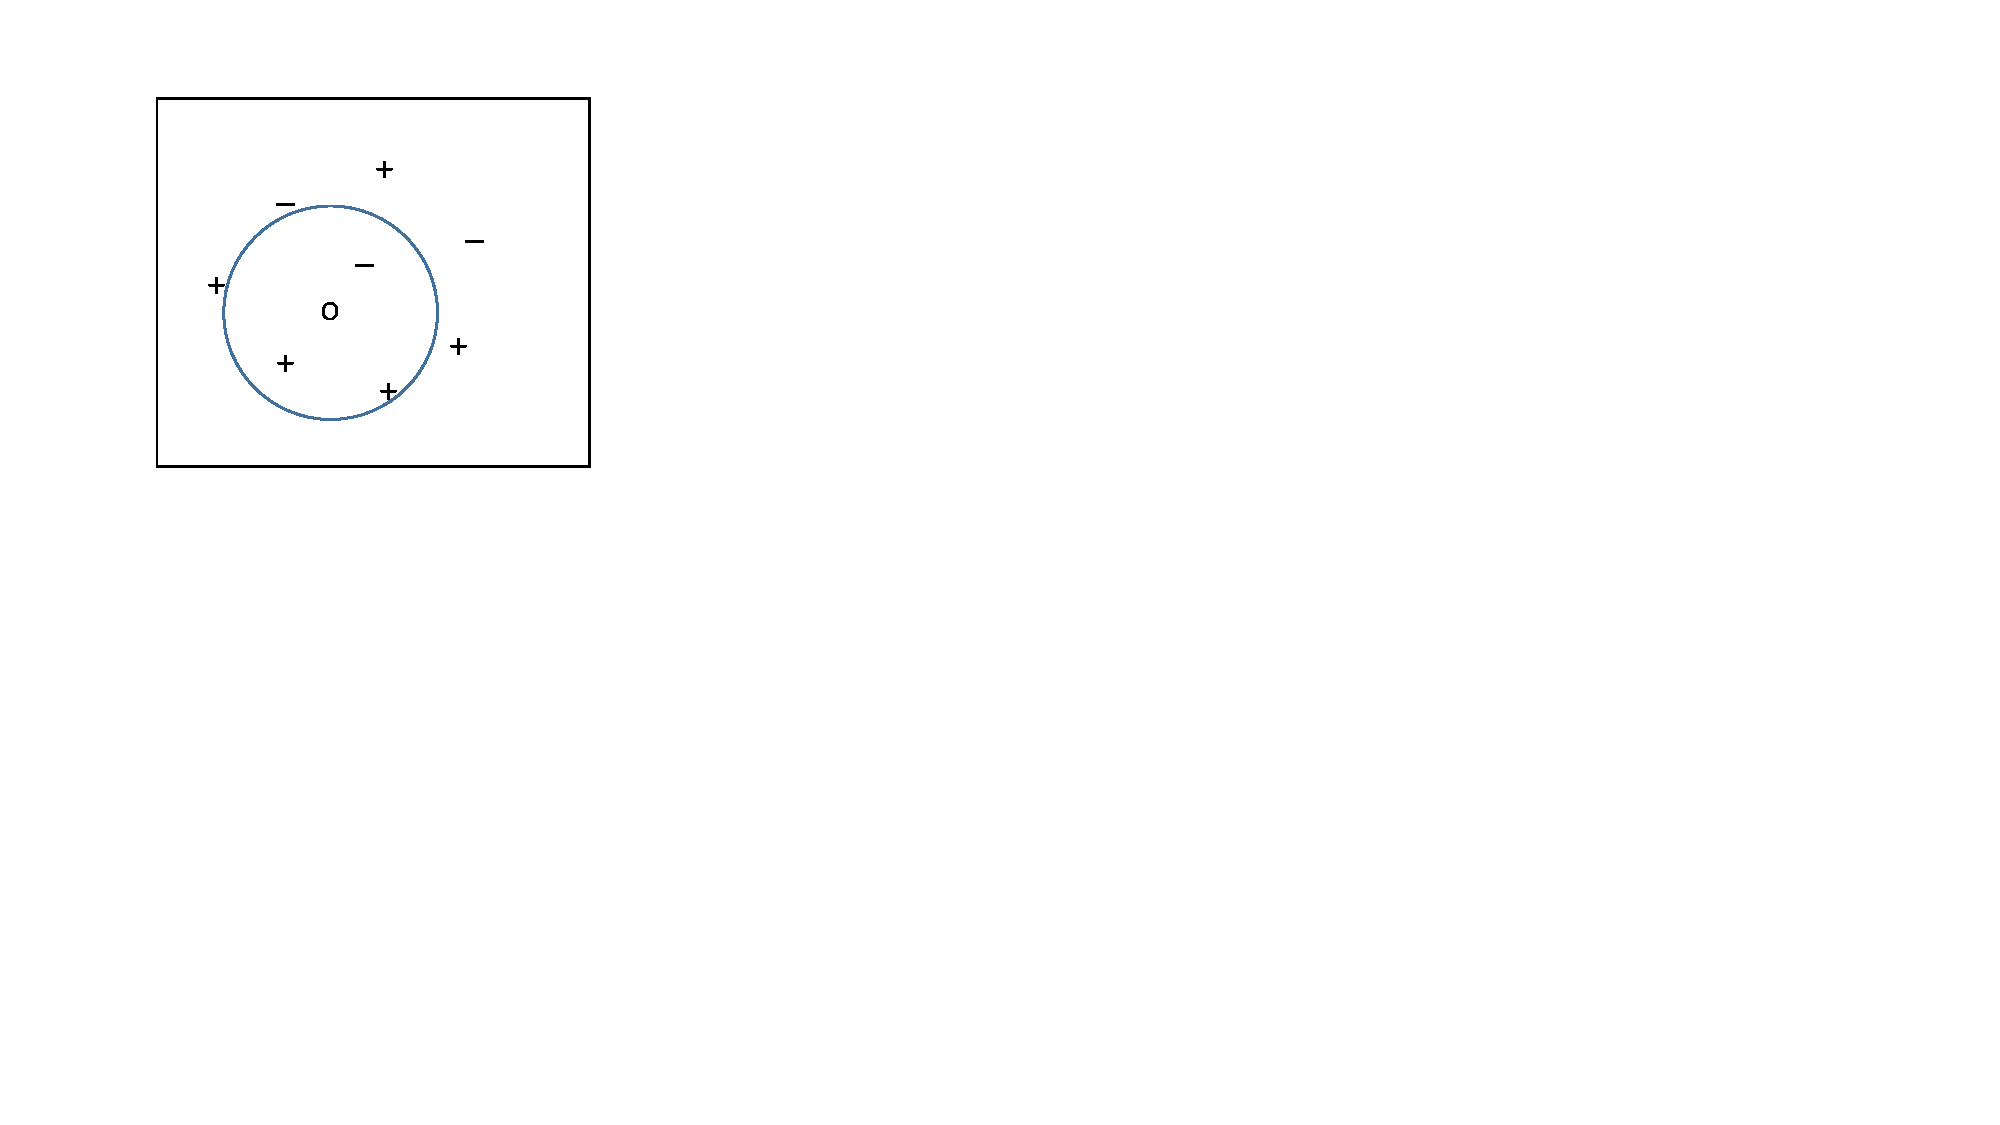
\includegraphics[width=3.0in]{figs/knn.pdf}
        \caption{Concept of $k$-NN}
        \label{fig:bg:knn}
    \end{center}
\end{figure}

Choosing an optimal $k$ is the prime challenge of $k$-NN algorithm, which is extremely training data dependent. Changing position of few training points could lead to a significant loss in performance. The method is particularly not stable in the class boundary. $k$ should be large enough that $k$-NN could overcome the noises in data, and small enough that instances of other classes are not included. Generally, higher $k$ reduces the overall noise and should be more precise. For most data set a value between $3$-$10$ performs much better than $1$-NN. Typically cross-validation is used to determine a good $k$. 

\subsection*{Na\"ive Bayes}
Naive Bayes classification is based on Bayes rule. Bayes rule says that the probability of event $x$ conditioned on knowing event $y$, i.e. the probability of $x$ given $y$ is defined as
\[
p(x|y) = \frac{p(x,y)}{p(y)} = \frac{p(y|x) p(x)}{p(y)}
\]
The naive Bayes classifier~\cite{langley92:nb} assumes that all the explanatory variables are independent. Given a feature set $X = x_1, x_2, \dots, x_n$ of $n$ independent variables, naive Bayes assigns the instances to $k$ possible outcome or classes, $p(C_k | X)$. Using Bayes rule, the conditional probability can be decomposed as:
\[
p(C_k |X) = \frac{p(C_k) p(X|C_k)}{p(X)}.
\]
In other words,
\[
posterior = \frac{prior \times likelihood}{evidence}.
\]
Using chain rule repetitively, it can be expressed as follows:
\[
p(C_k |X) = p(C_k) \prod_{i=1}^n p(x_i | C_k)
\]
The predicted class is the one which maximizes the conditional probabilities $p(C_k|X)$, that is, classifier assigns the class label $\hat{y} = C_k$ for some $k$ that satisfies:
\[
\hat{y} = \underset{k \in \{1, \dots, K\}}{argmax}  p(C_k) \prod_{i=1}^n p(x_i | C_k)
\]

\subsection*{Decision Tree}
Decision trees (DTs) are another popular genre of non-parametric supervised learning algorithms. Trees allow a way to graphically organize a sequential decision process. Decision tree, a directed acyclic graph, contains decision nodes, each with branches for all alternate decisions. Leaf nodes are labeled with respective class label. Each path from root to leaf is a decision rule, consisting of conditional part (unions of all internal nodes' conditions) and a decision (of leaf node).

Decision trees use {\it information gain} to select the splitting attribute that would maximize the total entropy of each of the subtrees resulting from the spit. Entropy is a measurement of purity of an attribute, typically ranged between 0 and 1. A pure attribute, attribute with definitive value-class relationship, would have a low entropy and is easy to predict. On the other hand attribute with highly mixed value-class relationship would yield high entropy. A common entropy function is-
\[
entropy = - \sum_{i=1}^n p_i \lg p_i.
\]
where $p_1, p_2, \dots, p_n$ are the distributions of several class attributes and $\sum p_i = 1$. Information gain is the difference between old and new entropy after a split. This is good measurement of relevance of an attribute. However, in cases where an attribute can take on a large number of distinct values, information gain is not ideal. Presence of large set of values could uniquely identify the classes but also reduces chance to generalize unseen instance and should be avoided to be place near root.

Decision tree is, however, computationally feasible. Average cost of constructing a decision tree for $n$ instances with $m$ attributes is $O(mn \lg n)$, and querying time is $O(\lg n)$.

\subsection*{Neural Network}
The Neural Network (NN) is a learning method inspired by biological neural network. A set of inter-connected nodes (also known as perceptrons and neurons) mimics biological neural network. Figure~\ref{fig:bg:nnlayer} shows a skeleton of a neural network. Neural network is a weighted directed graph where a input layer is connected to the output layer via some layers of hidden layers. This is commonly known as Multi-Layer Perceptron (MLP). Decisions are made looking only into the output layer only. Hidden layers enlarge the space of hypotheses. If there is no hidden layer, then neural network becomes a simple regression problem i.e. output is a linear function of inputs. Each connection among these nodes has an associated weight. Given an input data set, these weights are updated accordingly to best fit the classification model. Learning is done by back-propagation algorithm~\cite{raul96:nn}. Errors are propagated back from the output layer to the hidden layer and weights are updated to minimize error.
\begin{figure}[htbp]
    \begin{center}
        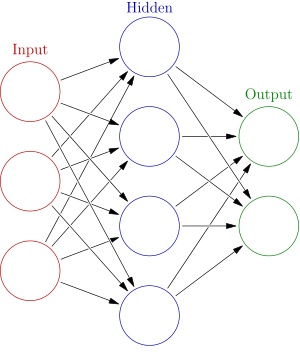
\includegraphics[width=4.0cm]{figs/nnlayers.png}
        \caption{Neural network layers}
        \label{fig:bg:nnlayer}
    \end{center}
\end{figure}

Learning starts with assigning a small value as initial weights to all the connection weights. In case of a single perceptron, learning process is analogous to moving a parametric hyperplane around. Let $w_i$ be the weight of $i$-th input, then after $t+1$ iteration weight $w_i(t+1) = w_i(t) + \nabla E_i(t)$, where $\nabla E_i$ is the gradient of the error function. For a input vector $\mathbf{x}$ and true output $y$, $E$ is defined as the squared error:
\[
E = \frac{1}{2} Err^2 = \frac{1}{2} (y - h_w(\mathbf{x}))^2
\]
Thus gradient of $E$ would be:
\begin{align*}
    \nabla E = \frac{\partial E}{\partial W_j} & = Err \times \frac{\partial Err}{\partial W_j} = Err \times \frac{\partial}{\partial W_j} (y - g(\sum_{j=0}^n w_j x_j)) \\
    & = - Err \times g^{\prime} (in) \times x_j
\end{align*}
Based on this, weight update rule would be:
\[
w_j = w_j + \alpha \times Err \times g^{\prime} (in) \times x_j
\]
where $\alpha$ is learning rate coefficient. Back propagation algorithm for multi-layer perceptron also works in similar fashion. Weights in the output layer are updated using following equation:
\[
w_{j,i} = w_{j,i} + \alpha \times a_j \times \nabla_i
\]
where $\nabla_i = Err \times g^\prime(in_i)$. Hidden layers propagates this error from the output layer using:
\begin{align*}
    \nabla_j &= g^\prime (in_i) \sum_i w_{j,i} \nabla_i \\
    w_{k, j} &= w_{k, j} + \alpha \times a_k \times \nabla_j
\end{align*}

MLP is a very expressive method. Only $1$ hidden layer is sufficient to represent all continuous functions and $2$ can represent any functions. MLP is prone to local minima, which is avoided by running MLP multiple times with different initial weight settings.
\clearpage

\chapter{Census Income Dataset}
\label{appndx:ci}

Census income data set, also commonly known as adult data set has 48842 instances consisting of 14 attributes that maps to a binomial Income class (<=50K or >50K). Attributes are age, sex, education, occupation, work class, working hours, marital status, relationship, country, race, final weight, capital gain, and capital loss. 2809 instance have missing values for either occupation or work class or both.

Occupation, education, marital status are the most important attributes. They can sufficiently classify the instance with an accuracy within 1\% of the accuracy achieved using all attributes. Education attribute has 16 values from pre-school to doctorate. 66\% of the instances belong to high-school grad, some college, and bachelor. Occupation attribute has 15 values. Instances are distributed in more balanced way. Marital status attribute consist of values from married, never married, and other status. The target income class is skewed towards <=50K class with 76\% of the instance.

Five primary clusters can be found in this dataset. Cluster 1 being mostly student groups, still studying and earning <= 50K. Cluster 2 are the young professionals, just started their career, and mostly earning less than 50K. Cluster 3 are the people with white collar jobs. People with bachelor or more education here earns >50K. Cluster 4 are the people with blue collar jobs, mostly earning <=50K. Cluster 5 are females. In this group too, people with bachelor or more degree earns >50K.

Most batched leaning algorithm achieves about 80-83\% accuracy with about 85-88\% F1 value.